\documentclass[10pt,a4paper]{article}
\usepackage[utf8]{inputenc}
\usepackage{polski}
\usepackage{amsmath}
\usepackage{amsfonts}
\usepackage{amssymb}
\usepackage{graphicx}
\usepackage{hyperref}
\usepackage{listings}
\usepackage{color}


\author{Klaudia Czuba, Mateusz Koprucki}
\title{VetOS - system wsparcia kliniki weterynaryjnej}
\date{}
\begin{document}

\lstset{columns=fullflexible, basicstyle=\ttfamily,xleftmargin=-2.5cm,frame=lr,framesep=2pt,framerule=0pt,showspaces=false,
inputencoding=utf8x, 
extendedchars=\true,
literate={ą}{{\k{a}}}1
{Ą}{{\k{A}}}1
{ę}{{\k{e}}}1
{Ę}{{\k{E}}}1
{ó}{{\'o}}1
{Ó}{{\'O}}1
{ś}{{\'s}}1
{Ś}{{\'S}}1
{ł}{{\l{}}}1
{Ł}{{\L{}}}1
{ż}{{\.z}}1
{Ż}{{\.Z}}1
{ź}{{\'z}}1
{Ź}{{\'Z}}1
{ć}{{\'c}}1
{Ć}{{\'C}}1
{ń}{{\'n}}1
{Ń}{{\'N}}1}
	
	\maketitle
	\newpage
	\tableofcontents
	\newpage
	
	\section{Wstęp}
	Przedmiotem dokumentacji jest system wsparcia kliniki weterynaryjnej przygotowany na zajęcia laboratoryjne z systemów baz danych. Autorami systemu są:
		\begin{itemize}
			\item Klaudia Czuba
			\item Mateusz Koprucki
		\end{itemize}
	System został zaprojektowany w formie aplikacji webowej do stworzenia której użyto następujących technologii:
		\begin{itemize}
			\item Serwer www - Apache2 wraz z PHP
			\item Serwer bazodanowy - Mysql 5.6.15
			\item System zarządzania treścią (CMS) Wordpress 4.7 z rozszerzeniami
		\end{itemize}
\newline
	Do celów demonstracyjnych aplikacja posiada trzy konta:
		\begin{itemize}
			\item vet\_test, hasło vet\_test - do prezentacji grupy weterynarzy
			\item staff\_test, hasło staff\_test - do prezentacji grupy obsługi
			\item admin\_test, hasło  admin\_test - do prezentacji możliwości administracji
		\end{itemize}
	W dokumentacji zamieszczono kody źródłowe SQL ze zmiennymi PHP np. 
	\begin{itemize}
		\item '.\$zmienna.'
		\item '\$zmienna'
	\end{itemize}
\newline		
		Pełne repozytorium dostępne jest pod adresem: 
	
	\url{https://github.com/zaknaifen/vetos_core}
	
	\section {Instalacja}
		W celu zainstalowania systemu należy zainstalować na serwerze lub komputerze lokalnym środowisko
		\begin{itemize}
			\item Dla Windows: Webserv 2.2
			\item Dla Linux: apache2 z php i mariadb.
		\end{itemize}
	Następnie ściągnąc repozytorium z adresu podanego we wstępie do lokalizacji środowiska. Z folderu sql wgrać poprzez phpmyadmin lub konsole mysql plik sql z bazą danych. 
	
	
	
	
	
	\section {Użytkownicy}
		Aplikacja pozwala na przypisanie do systemu wiele kont przez administrację z podziałem na grupy zdefinowane przez twórców aplikacji. Są to:
		\begin{itemize}
			\item Weterynarz (vet) - grupa przeznaczona dla lekarzy, pozwala na dostęp do modułu weterynaryjnej aplikacji
			\item Obsługa (staff) - grupa przeznaczona dla obsługi z dostępem do sekcji modułu obsługi
			\item Administratcja (admin) - grupa administracyjna, pełen dostęp do modułów. 
		\end{itemize}
	
	\section{Moduły}
	Aplikacja została podzielona na trzy główne moduły. 
	\subsection{Strona główna}
	Po uruchomieniu aplikacji ukazuje się strona główna z wiadomościami i aktualizacjami, w lewym górnym logu widnieje ikona do uruchomienia menu systemu. Dla użytkowników z grupy administracja będzie również widoczny podłużny pasek systemu CMS do zarządzania użytkownikami (tworzenie, modyfikowanie, usuwanie.)
	
	\includegraphics[width=11cm]1
	
	\newpage
	\begin{itemize}
		\item SQL wykorzystany dla tej strony:
	\begin{lstlisting}
		SELECT 
			news_tresc as NEWS, 
			news_data as DATA 
		FROM	 
			news 
		order by 
			news_data desc 
		LIMIT 10 ;
	\end{lstlisting}
	
	\end{itemize}

	\subsection{Moduł weterynarza}
	Moduł weterynarza jest dostępny dla użytkowników z grupy weterynarzy i administracji. Sekcja została podzielona na dwie części:
	\begin{itemize}
		\item $[W$] Grafik - przyszłe wizyty weterynarza, wraz z formularzem przejścia do konkretnej wizyty. 
		
		SQL wykorzystany dla tej strony:
		\begin{lstlisting}
		select 
			event_id as `Numer wizyty`,event_begin as `data`,
			event_time as `czas`,patient_id as `numer pacjenta`
		from 
			wp_calendar 
		where 
			vet_id=(select ID 
				from 
				wp_users 
				where user_login="'.$login .'")
		\end{lstlisting}
		
		\includegraphics[width=11cm]2
		\newpage
		
		Po wprowadzeniu numeru wizyty aplikacja przenosi użytkownika na stronę realizacji wizyty, gdzie:
			\begin{itemize}
				\item W części górnej pojawiają się dane pacjenta wraz z powodem wizyty
				\item W centralnej części znajduję się arkusz do wypełnienia podczas wizyty
					\begin{itemize}
						\item Diagnoza
						\item Zalecenia
					\end{itemize}
				
			\includegraphics[width=11cm]3
				
		SQL Wykorzystany dla tej strony:	
		\begin{lstlisting}
		select 
			patient_id as `numer pacjenta`, 
			patient_name as `imie pacjenta`, 
			patient_race as `rasa`,
			patient_birthdate as `data urodzenia`
		from 
			patient_info 
		where 
			patient_id=(select patient_id 
			from wp_calendar where event_id='.$visit_id.');
			
		---------------------------------------------------
		select 
			patient_health_card_id as `nr`,
			patient_health_card_date as `data`,
			patient_health_card_desc as `diagnoza`,
			patient_health_card_recom as `zalecenia`
		from 
			patient_health_card 
		where 
			patient_health_card_patient_id=(select patient_id 
				from wp_calendar 
				where event_id='.$visit_id.') 
		order by patient_health_card_date desc LIMIT 4;
		---------------------------------------------------
		SELECT 
			count(patient_health_card_id) 
		FROM 
			patient_health_card 
		where 
			patient_health_card_patient_id=(select patient_id 
				from wp_calendar 
				where event_id='.$visit_id.');
		---------------------------------------------------
		INSERT INTO 
			patient_health_card
			(patient_health_card_patient_id,
		 	patient_health_card_desc, 
		 	patient_health_card_recom, 
		 	patient_health_card_addby) 
		VALUES 
			((select patient_id 
				from wp_calendar 
				where event_id=18),
			'$visit_diag',
			'$visit_rec',
			'$login');
		
		
		
		
		\end{lstlisting}
		
			
				
				
				\item Z prawej strony wyświetlają się 4 ostatnie wpisy z historii wizyt pacjenta z możliwością przejścia do pełnej historii.
				
				
				\includegraphics[width=11cm]5
			
			\end{itemize}
	
		\newpage
		
		SQL Wykorzystany dla tej strony:
		
		\begin{lstlisting}
		select 
			a.vet_id,
			a.event_id as `numer wizyty`,
			a.event_begin as `data`,
			a.event_time as `godzina`,
			a.event_desc as `opis`,
			b.patient_id as `numer pacjenta`,
			b.patient_name as `imie pacjenta`,
			c.owner_name as `imie  wlasciciela`,
			c.owner_surname as `nazwisko wlasciciela`
		from 
			wp_calendar a
		join 
			patient_info b 
			on a.patient_id=b.patient_id
		join 
			owner_info c 
			on b.patient_id=c.owner_id
		where 
			(event_time>=curtime() 
			and a.vet_id=(select ID from wp_users 
		  		where user_login="'.$login.'") 
			and event_begin>=curdate())
		or 
			(event_begin>=sysdate()
			and a.vet_id=(select ID from wp_users
		  		where user_login="'.$login.'"))
		order by event_begin asc;
		\end{lstlisting}
		
		
		
		
		\item $[W$] Spis wizyt - strona pokazuje wszystkie wizyty przypisane do weterynarza, zarówno te przeszłe jak i przyszłe. 
	
		
		\includegraphics[width=11cm]4
		\newpage
		
		SQL Wykorzystany dla tej strony:
		\begin{lstlisting}
		select 
			event_id as `Numer wizyty`,
			event_begin as `data`,
			event_time as `czas`,
			patient_id as `numer pacjenta`
		from 
			wp_calendar where vet_id=(select ID 
				from wp_users 
				where user_login="'.$login.'")  
		order by event_begin  asc;
		\end{lstlisting}
			\end{itemize}
		
	\subsection{Moduł obsługi}	
		Moduł przeznaczony dla personelu odpowiedzialnego za zamówienia towarów, dodawania pacjentów i umawiania bądź ich anulacji. Sekcja została podzielona na cztery części. 
		
		\begin{itemize}
			\item $[S$] Wizyty - sekcja podzielona jest na 3 częsci:
			\begin{itemize}
				\item Kalendarz z podglądem dodanych wizyt.
				\item Formularze dodawania i anulowania wizyt oraz wyszukiwanie danych pacjentów.
				\item Listy dostępnych lekarzy.
			\end{itemize}
				\includegraphics[width=11cm]6
				\newpage
			
			SQL Wykorzystany dla tej strony:
			\begin{lstlisting}
			insert 
			into 
				wp_calendar 
				(event_begin,
				event_end,patient_id,event_title, event_desc, 
				event_time,event_recur,event_repeats,event_author,
				vet_id, event_active ) 
			values 	
				('$new_visit_date','$new_visit_date',
				'$new_visit_patient','Wizyta',
				'$new_visit_desc','$new_visit_time',
				'S','0','1','$new_visit_vet','1');
			---------------------------------------------------
			delete 
				from wp_calendar
			WHERE 
				event_id='$visit_number';
			\end{lstlisting}	
				
				
			
			
			 \item $[S$] Dodaj pacjenta - sekcja podzielona jest na 2 części:
			 \begin{itemize}
			 	\item Formularze dodawania właściciela i pacjenta.
			 	\item Formularz wyszukiwania danych właściciela, jeżeli już wcześniej się zarejestrował a dodaje kolejnego podopiecznego do systemu.
			 	
			 \includegraphics[width=11cm]7
			 \newpage
			 \end{itemize}
		 SQL Wykorzystany dla tej strony:
\begin{lstlisting}
		INSERT 
			INTO patient_info 
		SET patient_name='$npn', patient_race='$npr',
			patient_birthdate='$npbd', patient_owner_id='$npoi',
		    patient_addby='$login' 	 
		--------------------------------------------------- 
		SELECT 
			patient_id 
		FROM 
			patient_info 
		where 
			patient_addby="'. $login .'" 
		ORDER BY patient_id DESC LIMIT 1;	 
		---------------------------------------------------
		INSERT INTO owner_info 
		SET 
			owner_name='$non', owner_surname='$nos', 
			owner_phone='$nop', owner_address='$noa', 
			owner_addby='$login' "\end{lstlisting}	 
			 \item $[S$] Karta właściciela - sekcja wyświetla wszystkie dane właściciela oraz jego zwierząt
			 
			 \includegraphics[width=11cm]8
		
		SQL wykorzystany dla tej strony:
		\begin{lstlisting}
		select
			owner_id as `numer właściciela`, 
			owner_name as `imie`, 
			owner_surname as `nazwisko`, 
			owner_phone as `numer telefonu`, 
			owner_address as `adres` 
		from owner_info 
		where 
			owner_id="'. $owner_id . '" 
			or owner_surname="'. $owner_surname . '"
		---------------------------------------------------
		select 
			patient_id as `numer pacjenta`, 
			patient_name as `imie`, 
			patient_race as `rasa`, 
			patient_birthdate as `data urodzenia` 
		from owner_info a
		join patient_info b
		on a.owner_id=b.patient_owner_id
		where 
			owner_id="'. $owner_id . '" 
			or owner_surname="'. $owner_surname . '";
		\end{lstlisting}
			 
			 
			 \item $[S$] Dostępne materiały - sekcja przeznaczona do zamawiania towarów z dostępnej listy. Strona została podzielona na dwie części:
			 	\begin{itemize}
			 		\item Spis produktów
			 		\item Formularz dodawania i usuwania produktów do zamówienia i wysyłania gotowego zamówienia.
			 	\end{itemize}
		 	\includegraphics[width=11cm]9
		 	
		 SQL wykorzystany dla tej strony:
		 
		\begin{lstlisting}
		select 
			w.warehouse_id as `numer dostawcy`,
			s.warehouse_stock_id as `numer produktu`,
			i.warehouse_name as `nazwa`,
			s.warehouse_stock_name as `nazwa towaru`,
			s.warehouse_stock_desc as `opis`,
			s.warehouse_stock_value as `cena`,
			s.warehouse_stock_quant as `ilość w opakowaniu`
		from warehouse w
			join warehouse_info i 
				on w.warehouse_info_ID=i.warehouse_info_id
			join warehouse_stock s 
				on w.warehouse_info_ID=s.warehouse_id
		where warehouse_active="YES";
		---------------------------------------------------
		truncate vetos_core.order;
		---------------------------------------------------
		insert 
			into vetos_core.order_history 
				(order_id, warehouse_id,product_id,
				quantity,order_date,order_by) 
		select * from vetos_core.order;
		---------------------------------------------------
		INSERT 
		INTO vetos_core.order 
		SET 
			warehouse_id='$nov', product_id='$noa',  
			quantity='$noq', order_time='$time', order_by='$login'; 
		---------------------------------------------------
		delete from vetos_core.order 
			order by order_id desc limit 1;
		
		
		\end{lstlisting} 
		 
		 
		\end{itemize}
\subsection {Moduł administracji}
Sekcja została podzielona na sześć części:
	\begin{itemize}
		\item $[A$] Przeglądaj zgłoszenia - strona odpowiedzialna za wyświetlanie aktualnie otwartych zgłoszeń technicznych. Na dole strony znajduje się formularz przejścia do konkretnego zgłoszenia po wpisaniu numeru porządkowego zgłoszenia.
		
		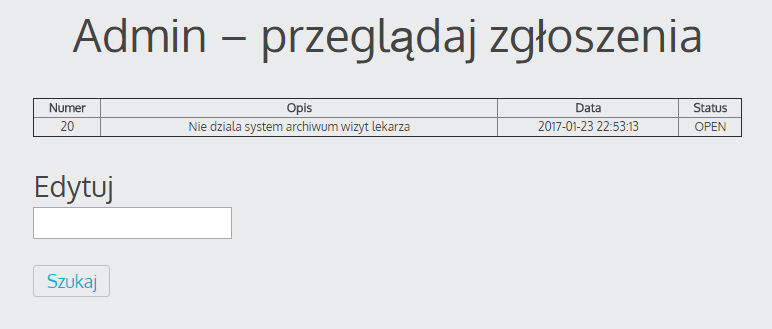
\includegraphics[width=11cm]{10}
		\newpage
		SQL wykorzystany dla tej strony:
		\begin{lstlisting}
		select 
			INC_id as Numer, 
			INC_description as Opis, 
			INC_date as Data, 
			INC_status as Status 
		from 
			incidents_main 
		where  
			INC_status="OPEN";
		\end{lstlisting}
		
		\item $[A$] Szukaj zgłoszenie - formularz do wyszukiwania, wyświetlania i edycji zgłoszeń zarówno otwartych jak i zamkniętych.
		
			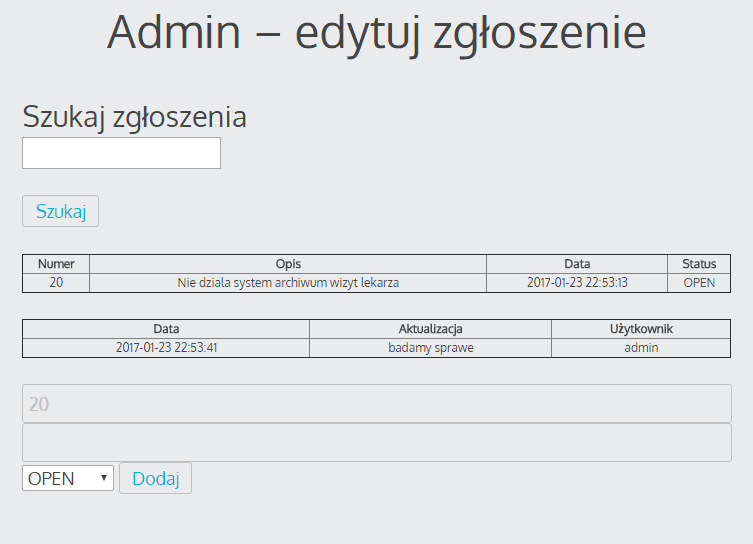
\includegraphics[width=11cm]{11}
		
		SQL wykorzystany dla tej strony:
		\begin{lstlisting}
		select 
			INC_id as Numer, 
			INC_description as Opis, 
			INC_date as Data, 
			INC_status as Status 
		from 
			incidents_main 
		where 
			INC_id='. $ticket . ';
		---------------------------------------------------
		SELECT 
			b.incidents_log_time as Data, 
			b.incidents_log_text as Aktualizacja, 
			b.incidents_log_user as Użytkownik 
		FROM 
			incidents_main a 
		INNER JOIN 
			incidents_log b 
			ON a.INC_id=b.incidents_log_ticket 
		where 
			a.INC_id='. $ticket . ' 
		order by 
			b.incidents_log_time ASC; 
		---------------------------------------------------
		INSERT INTO 
			incidents_log 
		SET 
			incidents_log_user='$login', 
			incidents_log_text='$ticket_desc', 
			incidents_log_ticket='$ticket', 
			incidents_log_time='$created_date' 
		---------------------------------------------------
		UPDATE 
			incidents_main 
		SET 
			INC_status = '$ticket_desc_status' 
		where 
			INC_id='$ticket'
		\end{lstlisting}
		
		
		\item $[A$] Archiwum zgłoszeń - strona wyświetlająca wszystkie zamknięte zgłoszenia. Na górze strony znajduje się formularz wyszukania zgłoszenia.
		
	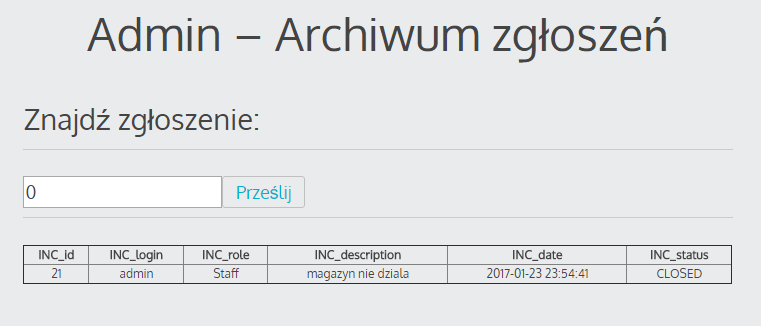
\includegraphics[width=11cm]{12}
		
		SQL wykorzystany dla tej strony:
		\begin{lstlisting}
		select 
			INC_id,INC_login,
			INC_role,INC_description,
			INC_date,INC_status 
		from 
			incidents_main 
		where INC_status="CLOSED" 
		LIMIT 30;
		\end{lstlisting}
		\newpage
		\item $[A$] Dodaj news - strona zawiera formularz dodawania wiadomości do głównej strony. 
		
		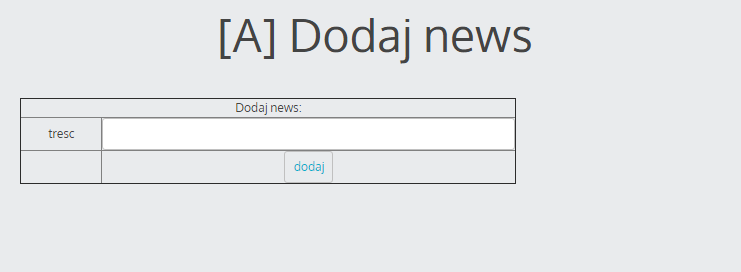
\includegraphics[width=11cm]{13}
		
			SQL wykorzystany dla tej strony:
		\begin{lstlisting}
		INSERT INTO 
			news 
		SET 
			news_tresc='$nn'; 
		\end{lstlisting}
		
		\item $[A$] Dostawcy - strona wyświetlająca wszystkich dostawców dla kliniki. 
		
		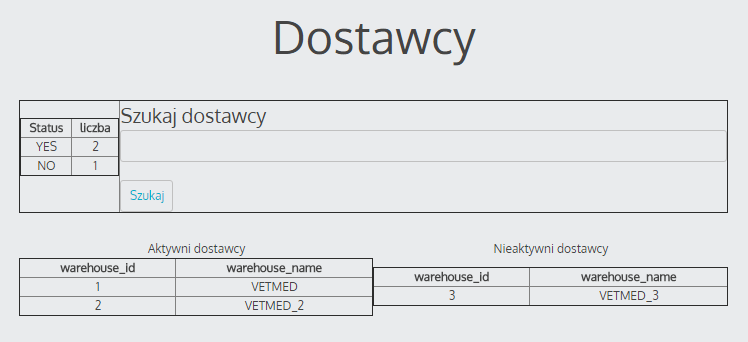
\includegraphics[width=11cm]{14}
		
		Sekcja została podzielona na dwie części:
			\begin{itemize}
				\item Formularz wyszukania dostawcy i przejścia do jego edycji (aktywacji bądź deaktywacji dostawcy oraz usunięcia dostępnego produktu z listy dostawcy).
					
					OBRAZEK! edycja dostawcy
				
				\item Podsumownia aktywnych i nieaktywnych dostawców
				\end{itemize}
		
		SQL wykorzystany dla tej strony:
		\begin{lstlisting}
		select 
			warehouse_active as Status,
			count(*) as liczba 
		from 
			warehouse 
		group by 
			warehouse_active desc;
		
		select 
			a.warehouse_id,
			b.warehouse_name 
		from 
			warehouse a 
		inner 
			join warehouse_info b 
			on a.warehouse_info_ID=b.warehouse_info_id 
		where 
			a.warehouse_active="YES";
		---------------------------------------------------
		select 
			a.warehouse_id,
			b.warehouse_name 
		from 
			warehouse a 
		inner join 
			warehouse_info b 
			on a.warehouse_info_ID=b.warehouse_info_id 
		where 
			a.warehouse_active="NO";
		---------------------------------------------------
		delete from 
			warehouse_stock 
		where 
			warehouse_stock_id='$dav';
		---------------------------------------------------
		select 
			warehouse_name as nazwa , 
			warehouse_city as miasto , 
			warehouse_address as adres , 
			warehouse_tel as telefon 
		from 
			warehouse_info 
		where 
			warehouse_info_id='. $supplier . ' ;
		---------------------------------------------------
		SELECT 
			warehouse_stock_id as numer, 
			warehouse_stock_name as nazwa, 
			warehouse_stock_desc as opis, 
			warehouse_stock_value as cena, 
			warehouse_stock_quant as ilosc 
		from 
			warehouse_stock 
		where 
			warehouse_id='. $supplier . ' ; 
		---------------------------------------------------
		UPDATE 
			warehouse 
		SET 
			warehouse_active='$warehouse_status' 
		WHERE 
			warehouse_id='$supplier' 
		
		
		\end{lstlisting}
		
		
		\item $[A$] Dodaj artykuł - strona odpowiedzialna za dodawania nowych artykułów do dostawców w systemie. Sekcja została podzielona na dwie części:
		
			\begin{itemize}
				\item Formularz dodania nowego produktu
				\item Listy aktywnych dostawców
			\end{itemize}
		
	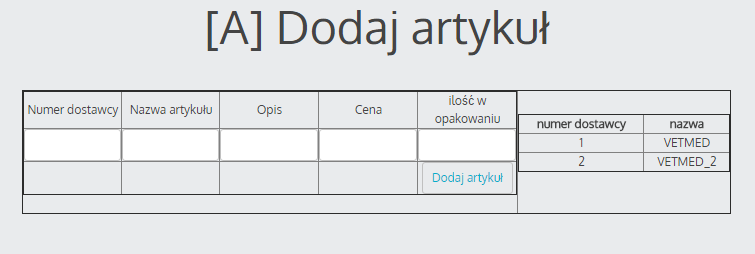
\includegraphics[width=11cm]{15}
		
		SQL wykorzystany dla tej strony:
		\begin{lstlisting}
		INSERT INTO 
			warehouse_stock 
		SET 
			warehouse_id='$nwsi', 
			warehouse_stock_name='$nwsa',  
			warehouse_stock_desc='$nwsd', 
			warehouse_stock_value='$nwsv', 
			warehouse_stock_quant='$nwsq' 
		---------------------------------------------------
		select 
			a.warehouse_id as `numer dostawcy`,
			b.warehouse_name as `nazwa`
		from 
			warehouse a 
		join 
			warehouse_info b 
			on a.warehouse_info_ID=b.warehouse_info_id 
		where 
			a.warehouse_active="YES";
		\end{lstlisting}
		
	\end{itemize}
\newpage
\subsection{Moduł zgłoszeń}
	Moduł odpowiedzialny za dodawanie i przeglądanie zgłoszeń technicznych dla użytkowników końcowych systemu. Strona została podzielona na cztery części:
	\begin{itemize}
		\item Szukaj zgłoszenia - formularz wyszukania i wyświetlenia szczegółów zgłoszenia
		\item Aktualne zgłosenia - lista otwartych zgłoszeń użytkownika
		\item Zamknięte zgłoszenia - lista zamkniętych zgłoszeń
		\item Formularz dodania nowego zgłoszenia
	\end{itemize}

	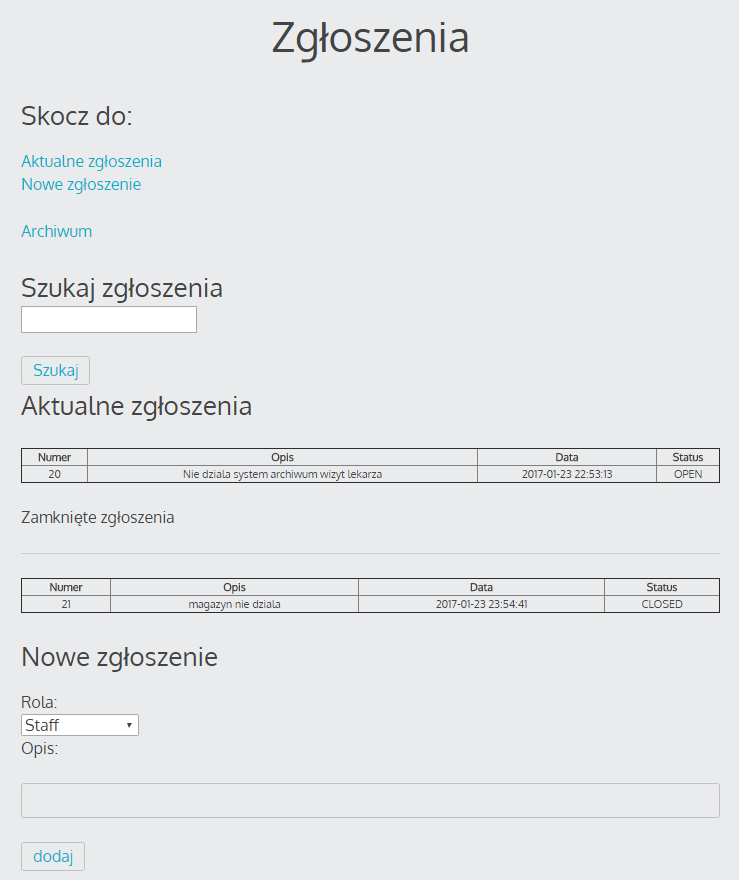
\includegraphics[width=11cm]{16}
	\newpage
	SQL wykorzystany dla tej strony:
	\begin{lstlisting}
	select 
		INC_id as Numer, 
		INC_description as Opis, 
		INC_date as Data, 
		INC_status as Status 
	from 
		incidents_main 
	where 
		INC_login="'. $login . '" 
		and INC_status="OPEN"; 
	---------------------------------------------------
	select 
		INC_id as Numer, 
		INC_description as Opis, 
		INC_date as Data, 
		INC_status as Status 
	from 
		incidents_main 
	where 
		INC_login="'. $login . '" 
		and INC_status="CLOSED"; 
	---------------------------------------------------
	INSERT INTO 
		incidents_main 
	SET 
		INC_login='$login', 
		INC_role='$role', 
		INC_description='$desc', 
		INC_date='$created_date', 
		INC_status='OPEN'; 
	
	
	\end{lstlisting}
	
\section{Spis tabel}
\begin{lstlisting}


	incidents_log         
	incidents_main         
	news                   
	order                  
	order_history          
	owner_info             
	patient_health_card    
	patient_info           
	test_inc               
	warehouse              
	warehouse_info         
	warehouse_stock        
	wp_calendar            
	wp_calendar_categories 
	wp_calendar_config     
	wp_cimy_uef_data       
	wp_cimy_uef_fields     
	wp_cimy_uef_wp_fields  
	wp_commentmeta         
	wp_comments            
	wp_links               
	wp_options             
	wp_postmeta            
	wp_posts               
	wp_signups             
	wp_term_relationships  
	wp_term_taxonomy       
	wp_termmeta            
	wp_terms               
	wp_usermeta            
	wp_users               
	wp_wpum_fields         
\end{lstlisting}
		
\end{document}